\section{Some existing Galant animations}
\label{app:galant_animations}

The purpose of these examples is mainly to illustrate the capabilities of
Galant. Many other algorithms are easily animated and some, such as
breadth-first search and Kruskal's minimum spanning tree algorithm have
already been implemented.

\subsection{Depth-first search}

Fig.~\ref{fig:dfs} illustrates an animation of depth-first search.
The code, in the current version of Galant, requires a few (four to be exact) lines lines at the beginning to set up the global variable \verb$time$ and the arrays \verb$discovery$ and \verb$finish$.
See the programmer guide (Appendix~\ref{app:programmer_guide}) for more
detailed instructions on how to do this properly.

The animation follows the conventions of Cormen et al. --- tree edges are selected (shown as thick red lines) and non-tree edges are labeled as B = back edge,
F = forward edge, and C = cross edge.
White nodes, not yet visited,
are neither marked nor selected;
gray nodes, visited but the visit is not finished, are selected
(thick red boundary);
and black nodes, visit is completed, are both marked and selected (red boundary and gray fill).
Labels on nodes indicate the discovery and finish times, separated by a slash.

Note that the animation begins with the statement\\
\hspace{3em} \verb+setDirected(true)+\\
which ensures that the graph is displayed and treated as a directed graph.
Depth-first search on an undirected graph requires keeping track of parents of visited nodes
or distinguishes visited from unvisited edges.


\begin{figure}

\begin{minipage}{0.5\textwidth}
\small
\begin{verbatim}
function visit( Node v ) {
  globals.time++;
  discovery[ v.getId() ] = globals.time;
  beginStep();
  v.setLabel( "" + discovery[ v.getId() ] );
  v.selected( true );
  endStep();
  for_outgoing( v, e, w ) {
    beginStep();
    if ( ! w.isSelected() ) {
      e.setSelected(true);
       visit( w );
    }
    else if ( finish[ w.getId() ] == 0 ) {
      e.setLabel( "B" );  /* ancestor */
    }
    else if ( finish[ w.getId() ]
              > discovery[ v.getId() ] ) {
      e.setLabel( "F" );  /* descendant */
    }
    else {
      e.setLabel( "C" );
    }
    endStep();
  }
  beginStep();
  globals.time++;
  finish[ v.getId() ] = globals.time;
  v.mark();
  v.setLabel( "" + discovery[ v.getId() ]
              + "/" + finish[ v.getId() ] );
  endStep();
}

setDirected( true );

beginStep();
for_nodes( u ) {
    u.setLabel("");
}
for_edges( e ) {
    e.setLabel("");
}
endStep();

for_nodes( u ) {
    if ( ! u.isSelected() ) {
        visit( u, null );
    }
}

\end{verbatim}
\end{minipage}
\begin{minipage}{0.49\textwidth}
\centering

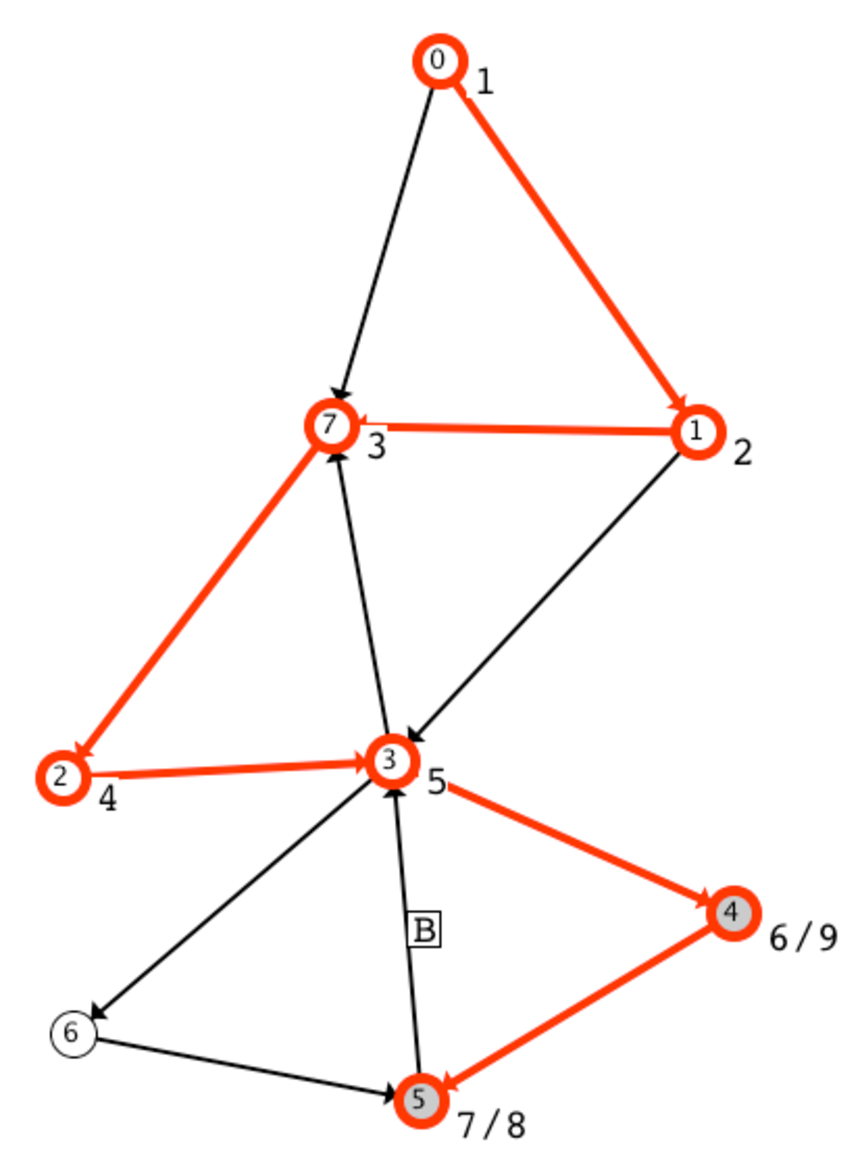
\includegraphics[scale=0.5]{X_dfs_d_1}

After first non-tree edge is labeled. 

\medskip

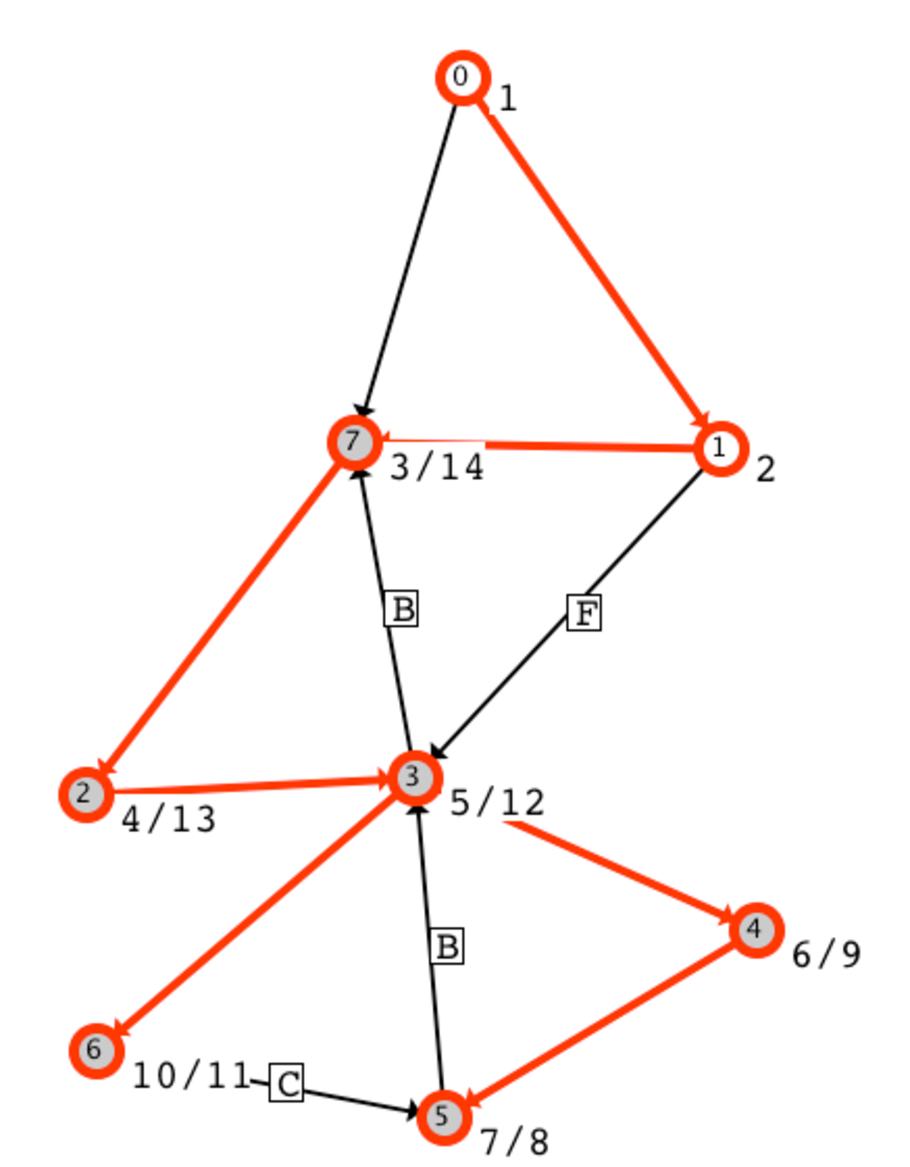
\includegraphics[scale=0.5]{X_dfs_d_2}

After all but one non-tree edges have been labeled.

\end{minipage}
\caption{Implementation of a depth-first search animation
  with an illustration of the graph panel during execution.}
\label{fig:dfs}
\end{figure}


Fig.~\ref{fig:dfs} illustrates an animation of depth-first search.
The code and definitions follow those of Cormen et al.~\cite{2009-Intro_to_Algorithms-Cormen}.
Tree edges are highlighted (selected)
and non-tree edges are labeled as \textbf{B}ack edges,
\textbf{F}orward edges or \textbf{C}ross edges.
White nodes, not yet visited,
are neither highlighted (selected) nor marked;
Gray nodes, visited but the visit is not finished, are highlighted only;
and black nodes, visit is completed, are both highlighted and 
marked.
Labels on nodes indicate the discovery and finish times, separated by a slash.

This particular algorithm, unlike our implementation of Dijkstra's,
is intended for a directed graph.
We would
need to write a different algorithm/animation
for undirected graphs.
When a graph is undirected an
edge is effectively directed both ways;
hence
tree
edges would get relabeled as back edges when they are encountered the second time.
The usual trick is to either mark edges if they have already been visited
or to keep track of the parent of a node when it is visited.


\subsection{Dijkstra's algorithm}

Fig.~\ref{fig:dijkstra} illustrates an animation of Dijkstra's shortest path algorithm.

\cmt{mention the role of node 0, the fact that decrease key is done in clumsy fashion to avoid a pointer into the queue (the actual decreaseKey function is not shown; not a big deal for small graphs, but
could be avoided if creator provided a binary heap implementation (which could
be an external class) and added an integer attribute.}

One of the simplest algorithms we have implemented is Dijkstra's algorithm
for the single source shortest paths problem.
Fig.~\ref{fig:dijkstra}
shows most of the implementation of the animation of Dijkstra's algorithm.
At every step the nodes already in the shortest path tree are \emph{visited}
(gray shading) and the nodes that have been encountered (but are not in the tree)
are \emph{selected }(thick red boundary).\footnote{
  Because these node and edge states both guide the logic of the algorithm
  and how the nodes/edges are displayed, the nomenclature has become awkward.
  A better way to handle the situation is to add initial declarations
  that specify color, thickness, and, in case of nodes, fill color, for each logical state.
  A logical state would have a name, e.g., \emph{InTree},
  and be automatically provided with a setter (Boolean argument),
  e.g., \emph{setInTree}, and a logical test, e.g., \emph{isInTree}.
}
Selected \emph{edges} (thick red) represent the current shortest paths to all
encountered nodes;
they are the edges of a shortest path tree when the algorithm is done.
The same algorithm animation
works for both directed and undirected graphs, as illustrated
in Figs.~\ref{fig:dijkstra_directed} and~\ref{fig:dijkstra_undirected}.
The user can toggle between the directed and undirected versions of a graph
via push of the appropriate button.
The functions \emph{beginStep} and \emph{endStep} define the points at which
the exploration of the algorithm stops its forward or backward motion.
In their absence, any state change (mark, select, change in weight, etc.)
constitutes a step, which, in some cases, can force the user
to do excessive ``stepping'' to move past uninteresting state changes.

\begin{figure}

\small
\begin{verbatim}
algorithm {
    NodePriorityQueue pq = new NodePriorityQueue();
    Edge [] chosenEdge = new Edge[nodeIds()]; 
    beginStep();
    for_nodes(node) {
        node.setWeight(INFINITY);
        pq.add(node);
    }
    Node v = getStartNode();
    setWeight(v, 0);
    endStep();

    while ( ! pq.isEmpty() ) {
        v = pq.removeMin();
        mark(v);        // nodes are marked when visited
        unHighlight(v); // and highlighted when on the frontier
        for_outgoing ( v, e, w ) {
            if ( ! marked(w) )  {
                if ( ! highlighted(w) ) highlight(w);
                double distance = weight(v) + weight(e);
                if ( distance < weight(w) ) {
                    beginStep();
                    highlight(e);
                    Edge previous_chosen = chosenEdge[id(w)];
                    if (previous_chosen != null )
                        unHighlight(previous_chosen);
                    pq.decreaseKey(w, distance);
                    chosenEdge[id(w)] = e;
                    endStep();
                }
            } // end, neighbor not visited (not in tree); do nothing if node
              // is already in tree
        } // end, adjacency list traversal
    } // stop when priority queue is empty
} // end, algorithm
\end{verbatim}

% \begin{verbatim}
% algorithm {
%     NodePriorityQueue pq = new NodePriorityQueue();
%     Edge [] chosenEdge = new Edge[nodeIds()]; 
%     beginStep();
%     for_nodes(node) {
%         node.setWeight(INFINITY);
%         pq.add(node);
%     }
%     Node v = getStartNode();
%     v.setSelected(true);
%     v.setWeight(0);
%     endStep();

%     while ( ! pq.isEmpty() ) {
%         v = pq.removeMin();
%         v.setVisited(true);
%         v.setSelected(false);
%         for_outgoing ( v, e, w ) {
%             if ( ! w.isVisited() )  {
%                 if ( ! w.isSelected() ) w.setSelected(true);
%                 double distance = v.getWeight() + e.getWeight();
%                 if ( distance < w.getWeight() ) {
%                     beginStep();
%                     e.setSelected(true);
%                     Edge previous_chosen = chosenEdge[id(w)];
%                     if (previous_chosen != null )
%                         previous_chosen.setSelected(false);
%                     pq.decreaseKey(w, distance);
%                     chosenEdge[id(w)] = e;
%                     endStep();
%                 }
%             } // end, neighbor not visited (not in tree); do nothing if node
%               // is already in tree
%         } // end, adjacency list traversal
%     } // stop when priority queue is empty
% } // end, algorithm
% \end{verbatim}

\caption{The implementation of the Dijkstra' algorithm animation.}
\label{fig:dijkstra}
\end{figure}


\begin{figure}[p]

\begin{center}
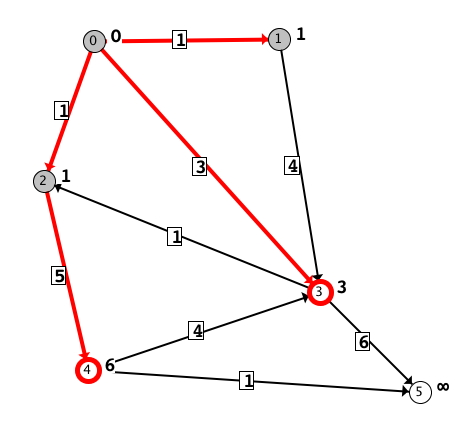
\includegraphics[scale=0.55]{X_dijkstra_directed}
\end{center}

\caption{Dijkstra's algorithm on a directed graph.}
\label{fig:dijkstra_directed}
\end{figure}


\begin{figure}[p]

\begin{center}
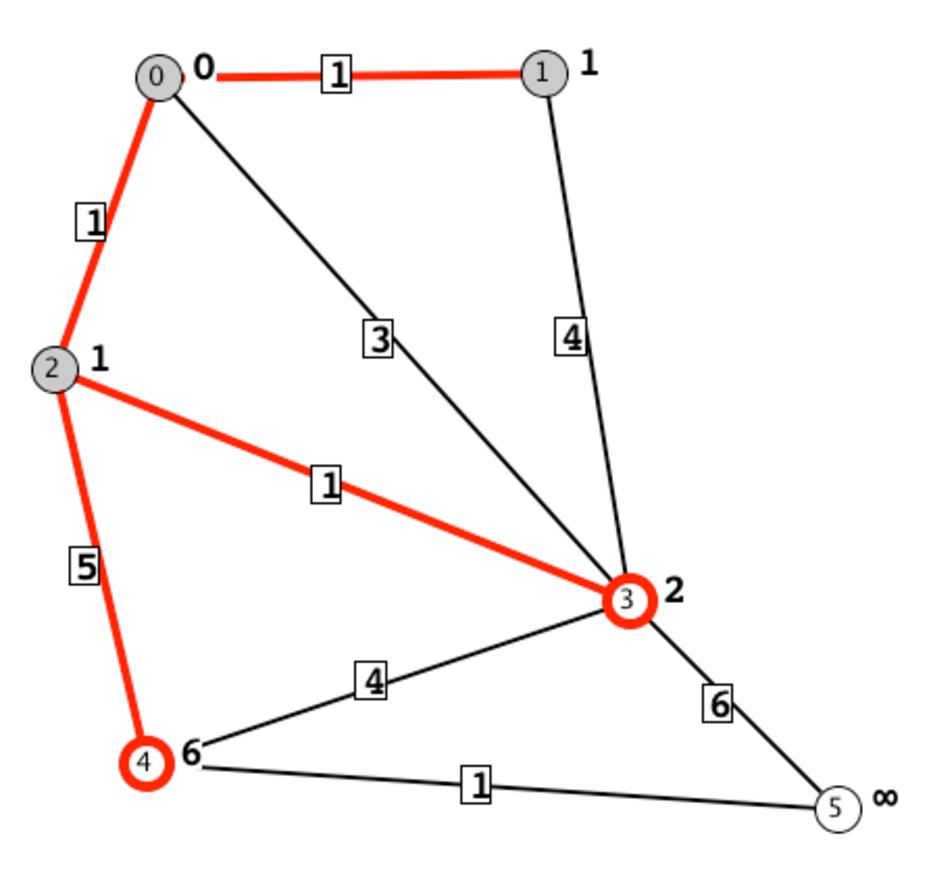
\includegraphics[scale=0.55]{X_dijkstra_undirected}
\end{center}

\caption{Dijkstra's algorithm on the same graph, undirected.}
\label{fig:dijkstra_undirected}
\end{figure}


The macro \emph{for\_outgoing($v,e,w$)}
creates a loop whose body is executed once
for each edge leading out of $v$; in the body, $e$ refers to the current edge
and $w$ to the other endpoint (any other variable names can be used).
In an undirected graph the term \emph{outgoing} applies to all incident
edges.\footnote{
Also provided are \emph{for\_incoming} and \emph{for\_adjacent};
the latter applies to all incident edges, even for directed graphs.
}

The difference between what the algorithm does on a directed versus an undirected graph is evident in the figures.
The edge \emph{from} node~3 to node~2 in the directed graph becomes an
edge \emph{between} the two nodes in the undirected form of the same graph.
Thus, in the undirected version, when node~2 is added to the tree
it also causes the distance from the source, node~0, to node~3 to be updated,
via the path through node~2.
These snapshots come from the executions of the \emph{same algorithm} on the
\emph{same graph}.
The only difference is that the explorer toggled from the directed to
the undirected
interpretation of the graph.

The array \verb+chosenEdge+ is required in order to control the highlighting.
Galant provides for seamless indexing of arrays with node id's: the
function \verb+nodeIds+ simply returns the largest node id plus one
(so that an array can be allocated correctly) and \verb+id(v)+ returns the
id of v, to be used as an index.
Node ids, therefore, need not be contiguous starting at 0, as,
in general, they won't be because of deletions or when graphs
come from external sources.




\subsection{Bubble sort}

% [Last modified: 2013 07 12 at 21:05:01 GMT]
